\chapter{Herramientas e infraestructuras utilizadas}
\label{cap:herramientas}


En este capítulo se realiza un breve análisis de las distintas herramientas e infraestructuras usadas a lo largo del proyecto.


%%%%%%%%%%%%%%%%%%%%%%%%%%%%%%%%%%%%%%%%%%%%%%%%%%%%%%%%%%%%%%%%%%%%%%%%%%%%%%%%
\section{Herramienta de gestión de configuración: Puppet}

Las herramientas de gestión de configuración tienen como objetivo describir y llevar a un sistema informático a un cierto estado. Normalmente esto suele incluir llevar a una serie de recursos (ficheros, usuarios, paquetes instalados, etc.) al estado deseado. Para cumplir esta misión se apoyan en dos conceptos básicos: iteración y convergencia. Estas herramientas tratan iteración tras iteración de acercar el sistema informático lo máximo posible al estado deseado. Es posible, por tanto, que el estado final no se alcance en una única ejecución, sino que sean necesarias varias ejecuciones.

Aunque esto pueda contrastar con el funcionamiento habitual de los programas (sería sorprendente que sólo se abriera medio editor de texto), no es tan excepcional en este entorno: si tenemos que poner en marcha dos servicios, de los cuales uno de ellos depende del otro, hasta que el primero no esté funcionando no podrá hacerlo el segundo. Una sola ejecución de la herramienta no serviría para poner ambos servicios en marcha, sino que serían necesarias dos iteraciones como mínimo. \\

Puppet \cite{puppetlabs} es una herramienta de gestión de configuración que posee un lenguaje declarativo (ver Anexo \ref{anx:puppet-language}) mediante el cual se especifica la configuración de los sistemas. A través de este lenguaje se especifica de forma declarativa los distintos elementos de configuración, que en la terminología de Puppet se llaman recursos. Mediante el uso de este lenguaje se indica en qué estado se quiere mantener el recurso y será tarea de Puppet el encargarse de que así sea. Cada recurso está compuesto de un tipo (el tipo de recurso que estamos gestionando), un título (el nombre del recurso) y una serie de atributos (los valores que especifican el estado del recurso). 

A la especificación de forma declarativa de los recursos y del estado que estos deben alcanzar se le denomina manifiesto. En general, un manifiesto contiene la información necesaria para realizar la configuración de un nodo. Un administrador de un sistema informático que use Puppet creará manifiestos en los que especifique los recursos y su estado. Por ejemplo, para crear un fichero el administrador escribirá en un manifiesto algo similar a lo siguiente:

%%% Revisar el salto de página
\pagebreak

\begin{lstlisting}
file {'testfile':
  path    => '/tmp/testfile',
  ensure  => present,
  mode    => 0640,
  content => "I'm a test file.",
}
\end{lstlisting}

Cuando se tiene listo el manifiesto a Puppet se le da la orden de aplicarlo. Los pasos que sigue para aplicarlo son:

\begin{itemize}
\item Interpretar y compilar la configuración.
\item Comunicar la configuración compilada al nodo.
\item Aplicar la configuración en el nodo.
\item Enviar un informe con los resultados.
\end{itemize}


Normalmente Puppet se ejecuta de manera periódica mediante un planificador de trabajos (por ejemplo, cron). Cada cierto tiempo contactará con el nodo que debe ser administrado y volverá a repetir los pasos anteriores. Es decir, Puppet está continuamente intentando llevar al nodo al estado especificado en el manifiesto. Si entre una ejecución y otra algo cambiara en el nodo, Puppet se daría cuenta e intentaría llevar al nodo al estado que le corresponde. \\

Aunque Puppet tiene la capacidad de actuar sobre un nodo distinto al nodo desde el que se aplica el manifiesto, a lo largo de este proyecto las ejecuciones de Puppet siempre serán sobre el nodo que aplica el manifiesto, siempre serán locales. Uno de los motivos para que esto sea así es que al ser un sistema distribuido con potencialmente muchos nodos es más sencillo si cada nodo posee el manifiesto que a él le corresponde en vez de que un único nodo alberge uno o dos manifiestos enormes en los que se especifique el sistema entero. Otro de los motivos es que la tolerancia a fallos es mejor cuanto menos se dependa de un nodo. \\

Dentro del ecosistema de Puppet hay una herramienta llamada MCollective \ref{anx:inst-mcollective}. Esta herramienta permite interactuar con grupos de máquinas y es especialmente útil cuando se quiere enviar una orden a varias máquinas en paralelo. La manera tradicional de implementar este tipo de comunicación es mediante un bucle de conexiones ssh, sin embargo, MCollective utiliza el patrón de mensajes editor/suscriptor. Hay varias tecnologías que implementan este patrón de mensajes, pero por simplicidad en este proyecto se usa RabbitMQ \ref{anx:inst-rabbitmq}.


%%%%%%%%%%%%%%%%%%%%%%%%%%%%%%%%%%%%%%%%%%%%%%%%%%%%%%%%%%%%%%%%%%%%%%%%%%%%%%%%
\section{Infraestructuras de ejecución de trabajos distribuidos}

En esta sección se analizan en profundidad las dos infraestructuras de ejecución de trabajos distribuidos usadas en este proyecto: AppScale y TORQUE.


%%%%%%%%%%%%%%%%%%%%%%%%%%%%%%%%%%%%%%%%%%%%%%%%%%%%%%%%%%%%%%%%%%%%%%%%%%%%%%%%
\subsection{Infraestructura AppScale}


AppScale es una implementación de código abierto del App Engine de Google. Al igual que App Engine, AppScale permite alojar aplicaciones web; a diferencia de App Engine, las aplicaciones no serán alojadas en la infraestructura que Google posee, sino que serán alojadas en una infraestructura que el usuario posea. Además de permitir alojar aplicaciones web, AppScale también ofrece las APIs de MapReduce y Neptune. El API de MapReduce permite escribir aplicaciones que hagan uso del \emph{framework} MapReduce. El API de Neptune añade a App Engine la capacidad de usar los nodos de la infraestructura para ejecutar trabajos. Los trabajos más representativos que puede ejecutar son: de entrada, de salida y MPI, aunque también se pueden ejecutar trabajos de otro tipo. \\

AppScale trata de imitar de la manera más fiel posible los servicios que ofrece el App Engine de Google, tratatando de alcanzar el mayor grado de compatibilidad con éstos. Como la tecnología que Google usa internamente en App Engine permanece oculta al público, AppScale tiene que hacer uso de otras tecnologías existentes para ofrecer las mismas funciones. En la Figura \ref{figure:tecnologias-appscale} \footnote[1]{Imagen obtenida de \url{http://code.google.com/p/appscale/wiki/Supported_AppEngine_APIs}} se puede ver toda la pila de tecnologías usadas en AppScale.

%\newpage % Si no se pone, la imagen aparece sola en una página entera.

\begin{figure} [!htbp]
  \centering
  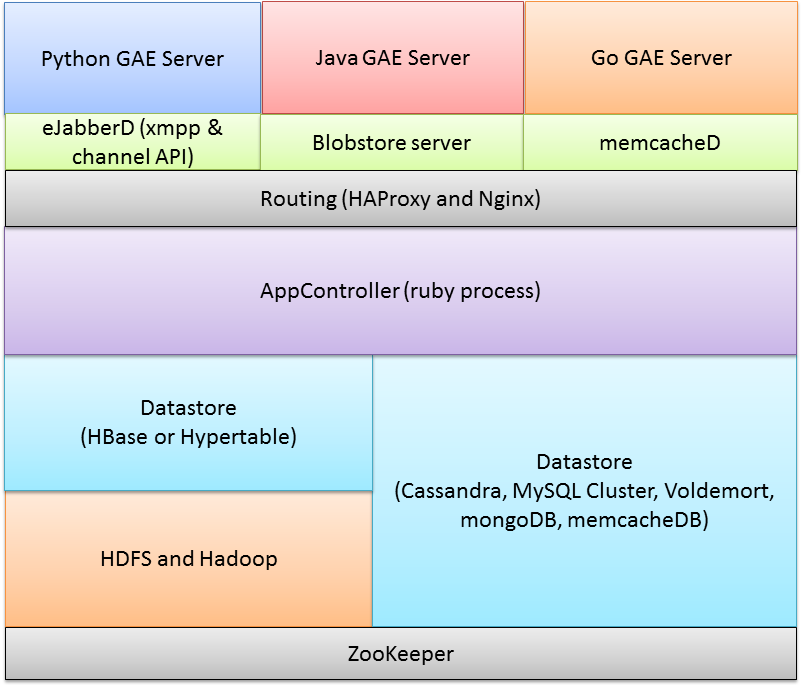
\includegraphics[width=13.5cm]{imagenes/AppScale_Stack.png}
  \caption{Tecnologías usadas por AppScale.}
\label{figure:tecnologias-appscale}
\end{figure}

Para permitir el alojamiento de aplicaciones web y la ejecución de trabajos una compleja infraestructura debe ponerse en marcha. Los distintos roles que un nodo puede desempeñar en una infraestructura de este tipo son los siguientes:

\begin{description}
\item[\texttt{Shadow}]: Comprueba el estado en el que se encuentran el resto de nodos.
\item[\texttt{Load balancer}]: Servicio web que lleva a los usuarios a las aplicaciones.
\item[\texttt{AppEngine}]: Aloja las aplicaciones web de los usuarios.
\item[\texttt{Database}]: Ejecuta los servicios necesarios para alojar a la base de datos elegida.
\item[\texttt{Login}]: Máquina desde la que se pueden hacer funciones administrativas.
\item[\texttt{Memcache}]: Proporciona soporte para almacenamiento en caché para las aplicaciones App Engine.
\item[\texttt{Zookeeper}]: Aloja los metadatos necesarios para hacer transacciones en las bases de datos.
\item[\texttt{Open}]: No ejecuta nada por defecto, pero está disponible en caso de que sea necesario.
\end{description}

Como muchos de estos roles suele desempeñarlos una máquina, se han creado unos roles agregados para facilitar el despliegue de la infraestructura. El rol \texttt{Controller} está compuesto por los roles Shadow, Load Balancer, Database, Login y Zookeeper; el rol \texttt{Servers} agrupa a los roles AppEngine, Database y Load Balancer; el rol \texttt{Master} está formado por los roles Shadow, Load Balancer y Zookeeper.

AppScale contempla la posibilidad de dos tipos de despliegue: por defecto y personalizado. En el despliegue por defecto un nodo sólo puede ser o bien \texttt{Controller} o bien \texttt{Servers}. En el despliegue personalizado el usuario es libre de especificar los roles de manera más precisa. Una especificación más detallada de los roles y de los despliegues puede encontrarse en el Anexo \ref{anx:appscale}.\\

Una vez puesta en marcha, la infraestructura de AppScale servirá tanto para alojar las aplicaciones web que el usuario despliegue como para ejecutar trabajos. Para desplegar las aplicaciones web hay que hacer uso de las AppScale Tools, un conjunto de herramientas que permiten, entre otras cosas, iniciar y terminar instancias, desplegar aplicaciones y eliminar aplicaciones. Para ejecutar trabajos hay que servirse, además de las AppScale Tools, del API de Neptune, que no es tan sencilla. En general, la ejecución de trabajos se consigue mediante tres pasos: en el primero se le indica el código fuente que se quiere subir a la infraestructura; en el segundo se le da la orden de ejecutar el trabajo; en el tercero se le piden los resultados de la ejecución. Cada uno de estos pasos debe indicarse, mediante un lenguaje específico de dominio, en un fichero que luego se interpretará con el programa Neptune. En el caso de un trabajo MPI, podemos definir, además del código a ejecutar, el número de máquinas sobre las que ejecutar el código y el número de procesos que se usarán para el trabajo.


%%%%%%%%%%%%%%%%%%%%%%%%%%%%%%%%%%%%%%%%%%%%%%%%%%%%%%%%%%%%%%%%%%%%%%%%%%%%%%%%
\subsection{Infraestructura TORQUE}

La otra infraestructura de ejecución de trabajos distribuidos que se ha elegido ha sido TORQUE, una de las infraestructuras clásicas en lo que a ejecución de trabajos se refiere. TORQUE permite a los usuarios la ejecución de trabajos \emph{batch} sobre un conjunto de nodos. Además de los nodos de computación necesarios para ejecutar los trabajos, una infraestructura de este tipo estará compuesta de un nodo maestro, que es el encargado de planificar la ejecución de los trabajos y de la gestión de los nodos de computación. \\

Una vez que la infraestructura está en funcionamiento los usuarios pueden mandar sus trabajos al nodo maestro. Éste, valiéndose de un planificador (en su versión más simple es una cola FIFO), decidirá a cuál de los nodos de computación le enviará el trabajo. El nodo de computación que reciba el trabajo será el encargado de ejecutarlo y de enviar los resultados de vuelta al nodo maestro una vez terminada la ejecución. \\

Además de contar con un planificador básico, TORQUE permite la integración con otros planificadores tanto comerciales (Maui Cluster Scheduler) como de código abierto (Moab Workload Manager) para mejorar la planificación de trabajos y la administración de los nodos del \emph{cluster}. A lo largo de este proyecto se usará, por simplicidad, el planificador más básico. \\

Para determinar qué usuarios son los que pueden enviar trabajos y qué usuarios son los que pueden realizar tareas administrativas, como por ejemplo cancelar un trabajo, TORQUE permite especificar dos grupos de usuarios: \texttt{managers} y \texttt{operators}. Para administrar el nodo maestro un usuario deberá pertenecer al primer grupo; para mandar trabajos deberá pertenecer al segundo. Por defecto únicamente el usuario \texttt{root} del nodo maestro puede administrarlo.


%%%%%%%%%%%%%%%%%%%%%%%%%%%%%%%%%%%%%%%%%%%%%%%%%%%%%%%%%%%%%%%%%%%%%%%%%%%%%%%%
\section{Herramienta de virtualización: KVM}


Una de las herramientas sobre las que se ha basado este proyecto ha sido la virtualización \emph{hardware} o virtualización de plataforma, que permite la simulación de un ordenador completo (llamado huésped) dentro de otro ordenador (llamado anfitrión). A la hora de hacer una virtualización \emph{hardware} hay varias opciones entre las que elegir, siendo las más ampliamente usadas Xen \cite{xen} y KVM \cite{kvm}. La principal diferencia entre ellas es que Xen ofrece paravirtualización mientras que KVM ofrece virtualización nativa. \\

La virtualización nativa permite hacer una virtualización \emph{hardware} completa de manera eficiente. Para ello, y a diferencia de la paravirtualización, no requiere de ninguna modificación en el sistema operativo de la máquina virtual; pero a cambio necesita un procesador con soporte para virtualización. KVM, que proporciona virtualización \emph{hardware}, está incluido como un módulo del núcleo de Linux desde su versión 2.6.20, así que viene incluido por defecto en cualquier sistema operativo con núcleo Linux. \\

Como los ordenadores del laboratorio poseen procesadores con extensiones de soporte para virtualización y sistema operativo Debian, se eligió KVM para dar soporte a las máquinas virtuales. Esto significa que se puede usar cualquier sistema operativo para las máquinas virtuales, sin necesidad de hacer ninguna modificación en el mismo. \\

Es importante recalcar que el proyecto fin de carrera no trata sobre la gestión de máquinas virtuales, sino que trata sobre la gestión de infraestructuras distribuidas. Así pues, la gestión de máquinas virtuales es una tarea necesaria para realizar la gestión de infraestructuras, pero no es la parte central.
